\section{Sparsity Test}
The computational cost of time integration can be reduced by several orders of magnitude by specifying the sparsity pattern of the Jacobian matrix. Because the spatial discretization relies on local neighborhood stencils, the resulting Jacobian matrix is highly banded (tridiagonal). 

In Figure \ref{fig:sparsity-test}, we compare the execution times of LSODA and BDF solvers using dense versus sparse Jacobians across varying grid resolutions \(N_x\). The test parameters are fixed at \(p = 2.5\), \(\varepsilon = 10^{-6}\), and \(T = 0.05\).

The results highlight two distinct computational regimes. For very small grids (\(N_x < 200\)), the dense implementation of BDF slightly outperforms its sparse counterpart. This is due to the inherent overhead required to allocate sparse data structures and track pointer indices, which dominates the execution time when the total number of operations is low. 

However, as \(N_x\) increases, the dense solvers exhibit \(O(N_x^3)\) scaling due to the dense LU factorization required during implicit solver steps. For example, doubling \(N_x\) from 1000 to 2000 in the dense LSODA solver increases the execution time by a factor of nearly eight (from 9.95s to 76.8s). Conversely, the sparse variants scale linearly, \(O(N_x)\). At the highest resolution tested (\(N_x = 2000\)), utilizing a sparse Jacobian in LSODA reduces the execution time from 76.8 seconds to 0.325 seconds, achieving a speedup of roughly \(236\times\). 

Furthermore, the data indicates that LSODA consistently outperforms the standard BDF implementation across all grid sizes for this specific parameter set, suggesting that LSODA's method-switching heuristics navigate the problem's stiffness more efficiently.

\begin{figure}[H]
  \centering
  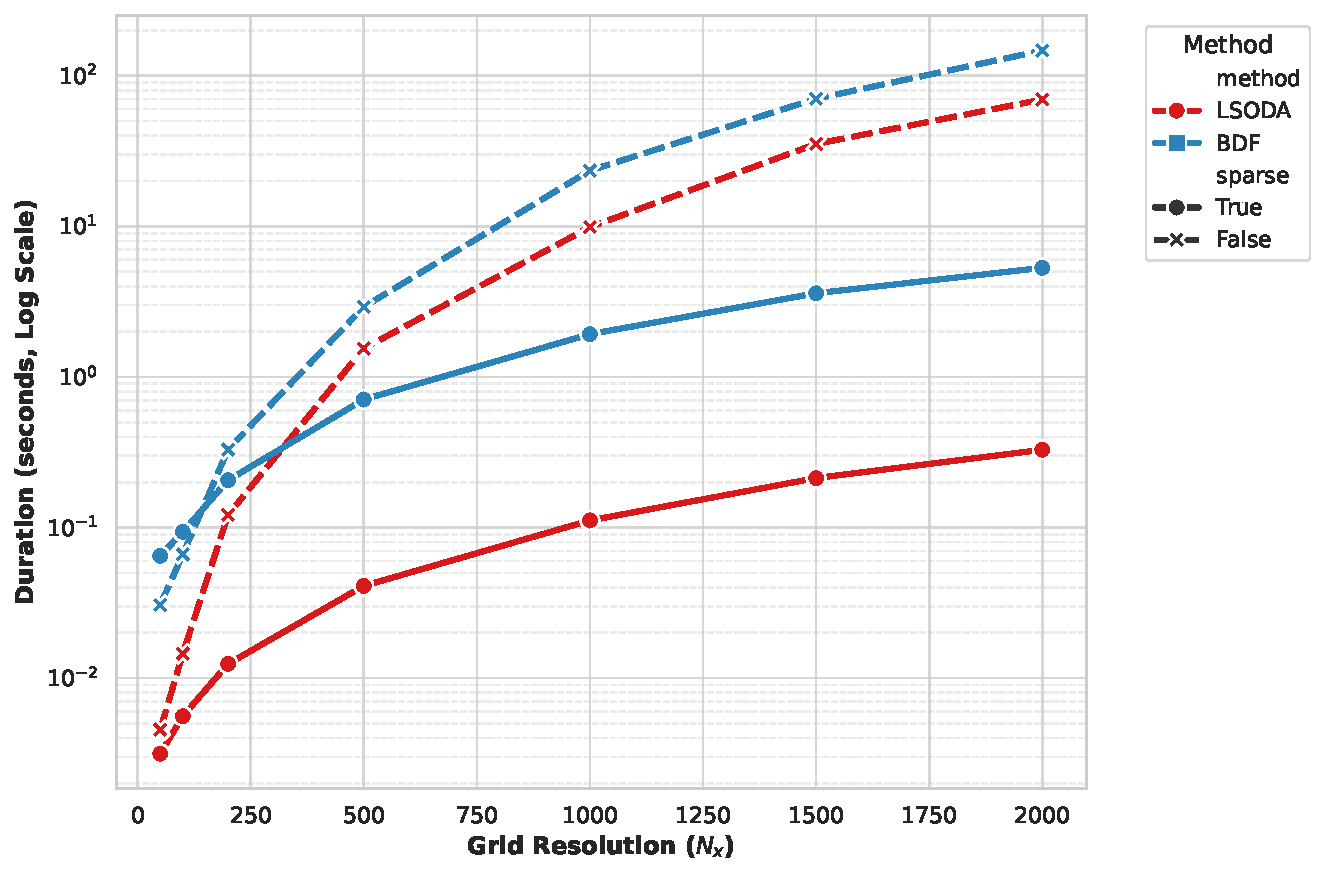
\includegraphics[width=\textwidth]{images/sparsity_scaling.pdf}
  \caption{Execution time scaling of LSODA and BDF solvers with dense and sparse Jacobians.}
  \label{fig:sparsity-test}
\end{figure}
